\documentclass[utf8,bachelor]{gradu3}
% If you are writing a Bachelor's Thesis, use the following instead:
%\documentclass[utf8,bachelor,english]{gradu3}

\usepackage{graphicx} % for including pictures

\usepackage{amsmath} % useful for math (optional)

\usepackage{booktabs} % good for beautiful tables

% NOTE: This must be the last \usepackage in the whole document!
\usepackage[bookmarksopen,bookmarksnumbered,linktocpage]{hyperref}

\addbibresource{references.bib} % The file name of your bibliography database

\begin{document}

\title{Lohkoketju - konsensus ja haasteet}
\translatedtitle{Blockchain - consensus and challenges}
\studyline{Tietotekniikka}
\avainsanat{%
  lohkoketju,
  konsensus-algoritmi,
  lohkoketjujen ongelmat
  }
\keywords{
    blockchain,
    consensus algorithm,
    blockchains problems
}
\tiivistelma{%

}
\abstract{%

}

\author{Niko Sihvo}
\contactinformation{\texttt{niko.m.sihvo@student.jyu.fi}}
% use a separate \author command for each author, if there is more than one
\supervisor{Tuomo Rossi}
% use a separate \supervisor command for each supervisor, if there
% is more than one

 % you don't need this line in a thesis
% \type{Template and manual for a thesis document class}

\maketitle


\begin{thetermlist}
\item[lohko] Lohkoketjun perustan muodostavien transaktioiden kokoelma.
\item[lohkoaika] Keskimääräinen aika mitä uuden lohkon luomiseen kuluu.
\item[node] Yksittäinen käyttäjä lohkoketjuverkossa
\item[louhija] Node, joka luo uusia lohkoja
\item[louhinta] Prosessi, jossa uusi lohko lisätään lohkoketjuun 
\item[DLT] Distributed Ledger Technology
\item[dApp] Decentralized Application
\item[NFT] Non-Fungible Token
\item[GDPR] The European General Data Protection Regulation
\end{thetermlist}

\mainmatter

\chapter{Johdanto}

Lohkoketjuteknologiat ovat saaneet viime vuosina huomattavan suosion, varsinkin kryptovaluuttojen muodossa. Lohkoketjuteknologiaa voidaan käyttää muihinkin kuin finanssialan toimiin, kuten logistiikkaan. 
Ideaalisessa tilanteessa lohkoketjut puoltaisi hajautettua, läpinäkyvää sekä demokraattisempaa internettiä.

Luvussa \ref{Lohkoketju} tarkastellaan lohkoketjun toimintaperiaatteita ja miten lohkoketjut on saanut lähtönsä.
\ref{Konsensus} luku tarkastelee pintapuolisesti potentiaalisia sekä suosituimpia konsensus-algoritmeja.
Lopuksi luvussa \ref{Haasteet} käydään läpi lohkoketjujen kohtaamia haasteita.



\chapter{Lohkoketju}\label{Lohkoketju}
\section{Historia}

Lohkoketjuteknologian perusajatus on lähtöisin 80- ja 90-luvun vaihteesta, jolloin Leslie Lamport kehitti Paxos protokollan. 
Tutkielmassa kuvaillaan konsensusmalli, missä verkko tietokoneita voivat tulla yhteisymmärrykseen epäluotettavassa ympäristössä \parencite{lamport2019part}. 
Vuonna 1991 otettiin käyttöön allekirjoitettu tietoketju elektronisena kirjanpitona dokumenttien digitaalisessa allekirjoittamisessa. Tietoketjusta nähtiin helposti kuka on muokannut dokumenttia digitaalisena jälkenä.

Nämä kaksi konseptia sovellettiin yhteen luoden ensimmäisen lohkoketjusovelluksen Bitcoinin. Bitcoin esiteltiin Satoshi Nakamoton artikkelissa \parencite{nakamoto2008bitcoin}.
Nakamoton artikkeli on monien modernien kryptovaluuttojen perusta.
Bitcoin on myös ensimmäisiä menestyneitä lohkoketjusovelluksia.


\section{Perusperiaatteet}

\begin{figure}[h]\centering
  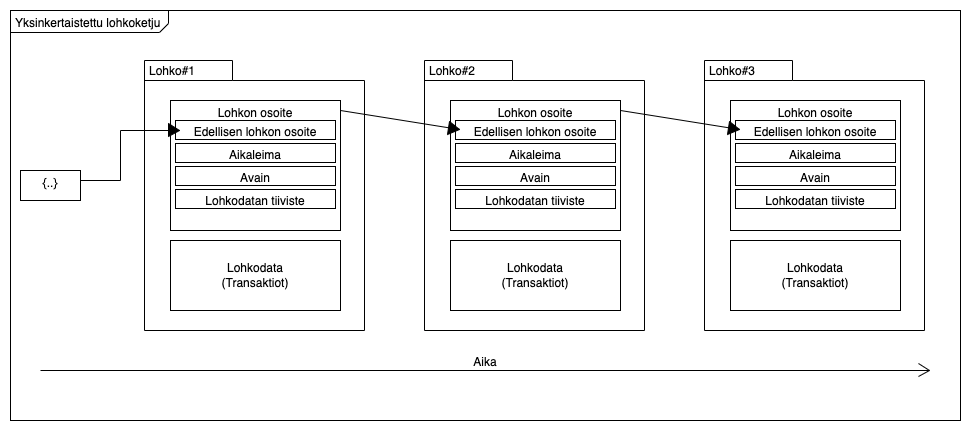
\includegraphics[height=7cm,keepaspectratio]{lohkoketjuDiag}
  \caption[Yksinkertainen lohkoketju]{Yksinkertainen lohkoketju}
  \label{fig:Lohkoketju}
\end{figure}

Lohkoketjut ovat hajautettuja digitaalisia tilikirjoja, jotka sisältävät lohkoihin ryhmiteltyjä kryptograafisesti allekirjoitettuja transaktioita \parencite{yaga2019blockchain}.
Jokainen lohko on linkitetty kryptograafisesti edelliseen validoinnin ja konsensuksen jälkeen lohkoon, mikä tekee lohkoista peukaloinnilta vapaan.
Kun uusia lohkoja liitetään ketjuun, vanhoja lohkoja on entistä vaikeampi muokata. 
Uudet lohkot toisinnetaan lohkoketjuverkon kopioiden kanssa ja mahdolliset konfliktit ratkaistaan automaattisesti käyttäen luotuja sääntöjä.

% Tee kaavio prosessista tähän

Lohkoketjun ensisijainen hyöty on mahdollistaa suorat transaktiot käyttäjien välillä ilman kolmansia osapuolia \parencite{yaga2019blockchain}.
Lohkoketjuissa yleisesti palkitkaan louhijoita eli käyttäjiä, ketkä julkaisevat uusia lohkoja ketjuun ja ylläpitävät tilikirjan kopiota.
Louhijoiden automatisoitu maksu mahdollistaa systeemin hajautetun hallinnon ilman kolmansia osapuolia.
Tämä lohkoketjujärjestelmän käyttäjien itsevalvottu mekanismi, konsensus-algoritmi, vakuuttaa, että vain validit transaktiot ja lohkot lisätään lohkoketjuun.
Lohkoketjujen käyttäminen mahdollistaa tilan, missä yksittäinen käyttäjä ei ohjaa transaktiota eikä järjestelmässä ole yksittäistä epäonnistumispistettä.

Yleisesti käyttäjät ovat pseudoanonyymeja, mutta heidän käyttäjätunnisteet eivät ole. 
Lisäksi kaikki transaktiot ovat julkisia. 
Koska lohkoketjutsovellukset ovat yleensä salattuja, on olennaista olla keinot luottamuksen luotiin ympäristössä, jossa käyttäjiä ei voi tunnistaa suoraan. 
Käyttäjä ei voi olla täysin anonyymi kuluttujansuojalakien takia \parencite{yaga2019blockchain}.
Perinteisesti käyttäjien välinen luottamus toteutetaan molempien osapuolien luottaman välikäden, kuten pankki, kautta.
Ilman luotettavia välikäsiä, lohkoketjussa luottamus luodaan seuraavan neljän avainominaisuuden kautta \parencite{zarrin2021blockchain}:

\begin{itemize}

\item Hajautus, missä jokainen lohkoketjuverkossa tehdyt transaktiot tehdään vain kahden noden välillä kerrallaan ilman kolmansia osapuolia. Hajautuminen mahdollistaa lohkoketjujen käytön ilman riippumattomia keskitettyjä viranomaisia. Tällöin jokaisella nodella on periaatteessa yhtäläiset äänestysoikeudet lohkoketjuverkossa

\item Muuttumattomuus viittaa siihen että transaktio täytyy validoida luotetuilla louhijoilla. Muuttumattomuus vakuuttaa, että nodeihin tallennetut tilikirjat pysyy absoluuttisina eikä niitä pysty poistamaan.


\item Anonymiteetti, viittaa jokaisen louhijan generoituun osoitteeseen uniikkina indentiteettinä. Vaikka kaikki lohkoketjut ei ole anonyymeja kokonaan ja jotkut harjoittaa pseudoanonymiteettiä, kuten Bitcoin ja Ethereum, missä osoitteet generoidaan jokaisessa lohkoketjun transaktiossa. 

\item Tarkastettavuus, missä jokaisella transaktiolla on oma viite lohkoketjussa, mikä on myös tallennettu lohkoketjun nodeihin. Näitä viitteitä käytetään jokaisen varmennetun transaktion aktivointiin ja jäljittämiseen lohkoketjussa. Näin jokaisesta transaktiosta jää merkki lohkoketjuverkkoon.
 
 \end{itemize}


\section{Komponentit}
Lohkoketjut sisältävät kolme pakollista pääkomponenttia, jotka ovat DLT, muuttumaton tilikirja ja konsensus-algoritmit \parencite{zarrin2021blockchain}.

DLT tarjoaa hajautetun tietokannan, joka muodostaa internetyhteyden käyttäjien välille. Tietokoneita joita käytetään yhteyksien luontiin kutsutaan nodeiksi.
Nodet sisältävät tilikirjan, joka on järjestetty lista aikaleimatuista transaktioista.
Tilikirjaa voi laajentaa vain tietokannalla, mikä mahdollistaaa turvallisen keinon jäljittää transaktoita ilman keskitettyä tarkastusta.

Muuttumattomalla tilikirjalla viitataan nodejen kykyyn olla muuttumatton.
Jokainen tilikirjaa on tallennettu jokaiseen nodeen ja tilikirjalla on viite itseensä lohkoketjussa muuttumattomana historiana.
Muuttumattomassa tilikirjassa käytetään salausfunktiota tilikirjojen eheyden ylläpitoon nodeissa.
Muuttumattomuus takaa etteivät muut välikädet pysty muokkaamaan transaktioiden sisältöä.

Konsensus-algoritmeja käytetään saavuttamaan yhteisymmärrys nodejen välillä, kun yritetään lisätä uutta lohkoa lohkoketjun loppuun.
Konsensus-algoritmi moderoi lohkoketjua sanelemalla nodeja kuinka päästä yhteisymmärrykseen ja päivittää lohkoketjuverkkoa. Lisää konsensus-algoretmeista luvusssa 5.

\section{Tiivistefunktio}
Lohkoketjut käyttävät tiivistefunktioita lohkojen ketjuttamiseen ja tiedon salaukseen. Jokaisella lohkolla on tiiviste osoitteena, mikä on generoitu lohkon sisällön mukaan. 
Tiiviste on yksisuuntainen kryptografinen funktio.
Tiivistefunktio ottaa yleisesti rajattoman määrän syötettä ja tulostaa lopulta tietyn pituisen merkkijonon. Jokainen tuloste on uniikki tietylle syötteelle.
Jos syötettä muutetaan merkilläkin, niin tuloste muuttuu täysin.
Täten jos lohkon sisältöä muuttaa, osoite muuttuu myös, mikä tekee validoiduista lohkoista muuttumattomia.


\section{Kategoriat}
Lohkoketjut voidaan kategorisoida kahteen joukkoon, luvattomiin ja luvallisiin.

Luvaton lohkoketjuverkko on kaikille avoin hajauttettu tilikirja-alusta. 
Jokainen käyttäjä pystyy liittämään uuden lohkon lohkoketjuun ilman ylempien tahojen lupaa. Yleisesti luvattomat lohkoketjut on avointa lähdekoodia.
Koska kaikilla luvattoman lohkoketjun käyttäjillä on lupa kirjoittaa lohkoketjuun on heillä myös oikeus lukea lohkoketjua.
Koska jokainen käyttäjä voi julkaista lohkoja luvattomassa lohkoketjussa, haitalliset käyttäjät voivat yrittää julkaista valheellista dataa lohkoketjuun.
Konsensus-algoritmi vaikeuttaa haitallisten käyttäjien yrityksiä korruptoida lohkoketjua huomattavasti.
Luvaton lohkoketjuverkko kannustaa yleensä ilkivallattomaan toimintaan palkitsemalla lohkojen julkaisijoita lohkoketjun omalla kryptovaluutalla.

Luvallisissa ketjuissa vain valitut käyttäjät voivat liittää lohkoja lohkoketjuun hajautetun tai keskitetyn viranomaisen toimesta.
Koska vain luvan saaneet käyttäjät ylläpitävät lohkoketjua, on mahdollista rajoittaa luku- ja kirjoitusoikeuksia.
Luvallisissa lohkoketjuverkoissa on samat ominaisuudet kuin luvattomassa lohkoketjussa.
Luvalliset lohkoketjut käyttävät siis myös konsensus-algoritmeja lohkojen liittämiseen, mutta yleensä käytössä ei ole yhtä raskaita algoritmeja, koska luvallisen lohkoketjun käyttäjillä on luottamusta toisiinsa. Luottamus perustuu siihen että käyttäjät ovat saaneet luvan lohkoketjuun ylemmältä taholta.

\section{Tyypit}

Lohkoketjun tyypin voi jakaa kolmeen joukkoon, julkinen, hybridi sekä yksityinen. Lohkoketjun tyyppi määrittelee ketkä osallistuvat varmennukseen ja konsensusprosessiin.

%\subsection{Julkinen lohkoketju}
Julkisessa lohkoketjussa jokainen osallistuja osallistuu lohkoketjun varmennukseen ja konsensusprosessiin. Julkinen lohkoketju on yleisesti luvaton lohkoketju, missä nodet voivat liittyä lohkoketjuun ilman erillisiä lupia. Nodeilla on täydet oikeudet lukea lohkoketjua ja kirjoittaa julkiseen lohkoketjuun.

%\subsection{Hybridilohkoketju}
Hybridilohkoketjussa vain valitut nodet julkisen tai yksityisen lohkoketjun haarasta pystyvät käsittelemään lohkoketjun varmennuksen ja konsensusprosessin. Hybridilohkoketju luokitellaan luvalliseksi lohkoketjuksi, koska se hyödyntää samaa logiikkaa todentamisessa, jossa vain rajatulla määrällä nodeja on luku- ja kirjoitusoikeudet.

%\subsection{Yksityinen lohkoketju}
Yksityinen lohkoketju käyttää yksityisiä nodeja organisaatiossa tai ryhmästä, joka on rajattu julkisuudelta, lohkoketjun varmennukseen ja konsensusprosessiin. Noden oikeuksia pystytään rajaamaan siten että node ei pysty osallistumaan molempiin prosesseihin, vaikka node kuuluisikin samaan organisaatioon tai ryhmään.  Yksityinen lohkoketju on luvallinen lohkoketju, mikä toimii samalla periaatteella valittujen nodejen kanssa kuten hybridilohkoketju. Se miten yksityinen lohkoketju eroaa hybridilohkoketjusta on siten että hybridimallissa nodet vahvistetaan useiden eri ryhmien toimesta, kun taas yksityisessä lohkoketjussa noden vahvistaa yksittäinen ryhmä, kuten organisaatio.

\begin{table}[ht]\centering
  \begin{tabular}{llll}
    \toprule
    Ominaisuudet & Julkinen & Hybridi & Yksityinen \\
    \midrule
    Konsensus & Kaikilla & Valituilla & Organisaatiolla \\
    Lukuoikeudet & Julkinen & Julkinen \& Yksityinen & Julkinen \& Yksityinen \\
    Muuttumattomuus & Lähes muuttumaton & Voidaan kajota & Voidaan kajota \\
    Tehokkuus & Matala & Korkea & Korkea \\
    Hajautuminen & Kyllä & Osittain & Ei \\
    Konsensus prosessi & Luvaton & Luvallinen & Luvallinen \\
    \bottomrule
  \end{tabular}
  \caption{Lohkoketjutyyppien vertailu - \cite{zarrin2021blockchain} - CC BY 4.0 - Muokattu}
  \label{tbl:cmdchange}
\end{table}

\section{Älysopimus}
Älysopimus on 1990 luvulla Nick Szabon esittelmä tietokoneprotokolla. Älysopimukset ovat ohjelmoituja sopimuslausekkeita, jotka toteutetaan, kun ennalta määritellyt ehdot täyttyvät.
Lohkoketjut mahdollistivat älysopimuksien käytön uudella tavalla, jossa sopimukset toteutetaan lohkoketjun päällä.
Jokainen älysopimuksessa suoritettu transaktio tallennetaan muuttumattomana lohkoketjuun, mikä tekee transaktioista jäljitettäviä ja peruuttamattomia. 
%Älysopimuksen elinkaari jakautuu neljään kohtaan. Luontiin, käyttöönottoon, suorittamiseen ja toteutumiseen.

% Tee kaavio

\chapter{Konsensus-algoritmit}\label{Konsensus}


Konsensus-algoritmi vaikuttaa lohkoketjun suorituskykyyn, hajautuvuuteen ja turvallisuuteen merkittävästi.
Konsensus-algoritmit voidaan jakaa kahteen joukkoon, todistus- ja äänestyspohjaisiin konsensus-algoritmeihin. 
Taulukko \ref{tbl:konsensus} sisältää listan konsensus-algoritemeista, jotka sopisivat parhaiten hajautetun internet käyttöön. 

\begin{table}[ht]\centering
  \begin{tabular}{lllll}
    \toprule
    Konsensus algortmi & Lohkoketju tyyppi & Lupatyyppi & Hajautuminen & DI \\
    \midrule
    PoW     & Julkinen \& Yksityinen 
            & Luvallinen 
            & Keskitasoinen 
            & Korkea \\
            
    PoAH    & Julkinen 
            & Luvallinen \& Luvaton 
            & Korkea 
            & Korkea \\
            
    PoP     & Julkinen \& Yksityinen 
            & Luvaton
            & Korkea 
            & Korkea \\
    \midrule
    PBFT    & Yksityinen  
            & Luvallinen
            & Keskitasoinen 
            & Korkea \\
            
    dBFT    & Yksityinen  
            & Luvallinen 
            & Keskitasoinen 
            & Korkea \\
            
    SCP \& ripple   
            & Yksityinen  
            & Luvaton
            & Keskitasoinen 
            & Korkea \\
    \midrule
    Paxos
            & Yksityinen
            & Luvallinen
            & Matala
            & Korkea \\
    Raft
            & Yksityinen
            & Luvallinen
            & Keskitasoinen
            & Korkea \\

    \bottomrule
  \end{tabular}
  \caption{Konsensus-algoritmit. \cite{zarrin2021blockchain} - CC BY 4.0 - Muokattu}
  \label{tbl:konsensus}
\end{table}

\section{Todistuspohjainen konsensus}
Todistuspohjaisissa konsensuksissa nodet kilpailevat keskenään laskemalla ja ratkaisemalla kryptograafista ongelmaa.
Se node, joka ratkaisee ongelman saa luvan laajentaa lohkoketjua.
Lohkon lisäyksen jälkeen alkaa uudelleen kryptografisen ongelman ratkominen.
Luvattomat lohkoketjut käyttävät yleensä todistuspohjaista konsensus algoritmia.

%\subsection{PoW - Proof-of-Work}
Proof-of-Work (PoW) on peräisin kryptovaluutoista, kuten Bitcoin ja Etherium. PoW algoritmi käyttää laskentatehoa kilpailuun, jossa nodet laskevat matemaattisia ongelmia. 
Kun joku node saa ratkaistua kierroksen ongelman, node saa palkinnoksi luoda uuden lohkon ketjuun ja yleisesti kryptovaluuttaa. Uusi kierros alkaisi, lisäten lohkoketjun pituutta rajattomasti. PoW algoritmin heikkous on sen energian kulutus ja suuren laskentatehon tarve. 
Ongelman haastavuus riippuu lohkoketjun saatavilla olevan laskentatehon mukaan myös lohkoketjun pituus vaikuttaa suhteellisesti työmäärään.

%\subsection{PoAH - Proof-of-Authentication}
Proof-ofAuthentication (PoAh) poistaa tarpeen käänteiselle tiivestefunktiolle, luoden energiatehokkaan lohkon todentamismetodin. PoAH:n todentamisprosessi varmentaisi lohkon ja lohkon alkuperän.
Node saisi täten luottamuspisteitä jokaisesta suoritetusta varmistetusta transaktiosta. Luottamusarvo on PoAh konsensus-algoritmin ydinosa.

%\subsection{PoP - Proof-of-Property}
Proof-of-Property (PoP) on kevyt ja skaalautuva konsensusprotokolla, mikä tarjoaa todistuksen tietorakenteiden ominaisuuksille. Tämä todistus on sidottu noden uniikkeihin osoitteisiin. Todistus tallentaa lohkoketjun tilan jokaiseen uuteen luotuun lohkoon. PoP on energiatehokas todistuksien arkitehtuurin takia, mikä vähentää nodejen tarvitseman informaation määrää transaktioiden toteuttamiseen.

\section{Bysanttinen äänestyskonsensus}
Bysanttiset äänestyskonsensukset perustuu siihen että node voi epäonnistua sekä lähettämään virheellisiä viestejä järjestelmään ja käyttäjälle. 
Bysanttiset äänestyskonsensukset ottavat konsensuksessa huomioon virheelliset viestit tai äänet äänestysprosessissa.

%\subsection{PBFT - Practical Byzantine fault tolerance}
Practical Byzantine fault tolerance (PBFT) tarvitsee kaikkien nodejen osallistumisen konsensusprosessiin.
PBFT:ssä konsensukseen päästään, kun 2/3 kaikista nodeista on äänestänyt samaa konsensusta.
Täten PBFT tarjoaa korkea suoritustehon, matalan latenssin, vähäisen energiankulutuksen verrattuna PoW konsensus-algoritmiin.
PBFT sisältää skaalautuvuusongelman luvattomassa lohkoketjussa sen aiheuttaman korkean tietoverkkorasituksen takia sekä sisältää matalan toleranssin väärinkäytölle.

%\subsection{dBFT - Delegated Byzantine fault tolerance}
Delegated Byzantine fault tolerance (dBFT) toimii lähes samalla tavalla kuin PBFT, mutta ei tarvitse kaikkien nodejen osallistumista äänestysprosessiin. Täten dBFT skaalautuu paremmin kuin edeltäjänsä PBFT.
dBFT algoritmissa tiettyjä nodeja valitaan edustamaan muita tai ryhmää nodeja.
Vaikka dBFt skaalautuu paremmin tietoverkoissa, niin sen suuri latenssi estää uusien lohkojen luomisen tehokkaasti.

%\subsection{SCP \& ripple - Stellar concensus protocol}
Stellar concensus protocol (SCP) käyttää PBFT-varianttia, missä nodeilla on vapaus luottaa toisiin nodeihin. Tämä luottamuksen vapautta käytetään konsensukseen pääsemisen prosessissa.
SCP tarjoaa korkeaa suoritustehoa ja vähäistä energiakulutusta, mutta kärsii tietoverkkorasitteesta, joka nostaa latenssia huomattavasti. 

Ripple on SCP:ta vastaava algoritmi, missä latenssia on saatu madallettua huomattavasti. Vaikka Ripple keskittyy ratkaisemaan latenssiongelmaa, Ripple on tarkoitettu rahallisiin tarkoituksiin, jolloin se ei sovi .

\section{Törmäys äänestyskonsensus}

Törmäykseen perustuvat algoritmit ovat bysanttilaisten algoritmien alakategoria, joka ohittaa törmäyksen epäonnistumisen. Törmäysalgoritmissa otetaan huomioon epäonnistuneet nodet. Erona bysanttilaisiin algoritmeihin on se, että törmäysalgoritmit eivät pysty ylläpitämään 100\% törmäystoleranssia.

%\subsection{Paxos}
Paxos on erittäin teoreettinen konsensusalgoritmi, minkä takia Paxosta on vaikea ymmärtää ja toteuttaa käytännössä \parencite{andrey2019review}.
Paxos-algoritmilla on 50\% törmäyssietokyky \parencite{panda2019study}.
Paxos on alunperin suunniteltu pienille suljetuille tietoverkoille. Tämän takia Paxos ei oikein sovellu internetkäyttöön.
Toisaalta Paxos-algoritmin äänestys- ja ankkurointijärjestelmä voisivat olla tietoturvallisia ominaisuuksia internetille. 
Paxos perustuu kahteen päärooliin, ehdottajaan ja äänestäjiin. Yksinkertaisettuna äänestäjät valitsevat ehdottajan ja ehdottaja vastaanottaa käyttäjien ehdotuksia.
Paxos-algoritmin suurin ongelma on makaa ehdottajassa, joka hallitsee äänestäjiä. Tämä ongelma tekee Paxos-algoritmista keskitetyn tapaisen, huolimatta mahdollisuudesta toteuttaa Paxos algoritmia hajautetulla tavalla. Kaaviossa \ref{fig:Paxos} on ilman virheitä tapahtunut yksinkertaistettu Paxos-algoritmin tilakaavio.


Raft-algoritmi yrittää tehdä Paxos algoritmista lähestyttävämmän ja helpommin ymmärrettävän. Raft saavuttaa saman suoritustehon Paxos, mutta pienemmällä 40\% törmäystoleranssilla \parencite{panda2019study}. 
Koska Raft on arkitehtuuriltaa samanlainen kuin Paxos, Raft sisältää saman keskitetyn hallitsevan johtajan ongelman.

\section{Käytettävyyden tarkastelu}
Parhaimmat vaihtoehdot hajautetulle internetille ovat PoP, Paxos ja PoAh konsensusalgoritmit \parencite{zarrin2021blockchain}. 
PoP tarvitsee vähän muistia ja laskentatehoa.
PoP-algoritmilla on yhteys semanttiseen teknologiaan tarjoamalla identiteetteja datarakenteiden ominaisuuksille.
Paxos on toinen hyvä vaihtoehto sovellettavuuden takia. Paxos algoritmia adaptoitu moniin erilaisiin järjestelmiin, mikä tekee Paxos-algoritmista hyvämaineisen uudelleenkohdennukseen.
Vaikka Paxos-algoritmin protokollaa ja toteutettavuutta on vaikea ymmärtää. Jotta Paxos olisi hyvä vaihtoehto hajautetulle internetille, tulisi algoritmia kehittää lohkoketjuja varten.
PoAH täyttää hajautetun internetin kriteerit olemalla vakaa, skaalautuva ja tarpeeksi tietoturvallinen. PoAH-algoritmin luottamusjärjestelmä on tehokas työväline luotettavien nodejen luomiseen samalla pitäen nodet samanarvoisina järjestelmässä

\begin{figure}[h]\centering
  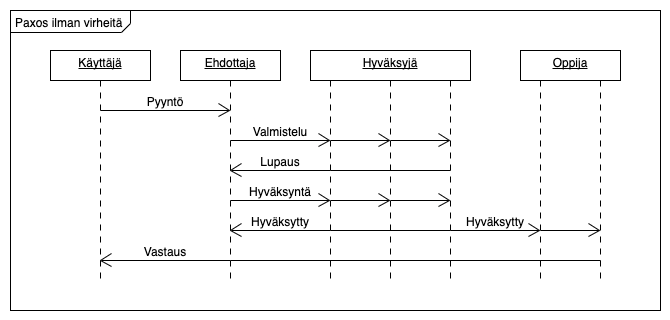
\includegraphics[height=6cm,keepaspectratio]{PaxosDiag}
  \caption[Yksinkertaistettu Paxos algoritmi]{Yksinkertaistettu Paxos algoritmi}
  \label{fig:Paxos}
\end{figure}

\chapter{Lohkoketjujen haasteet}\label{Haasteet}

\section{Hallinto ja sääntely}
Jos lohkoketjut otetaan globaalisti käyttöön, keskitetyt regulaatiojärjestöt, kuten hallinnoilliset järjestöt ja kansainväliset korporaatiot eivät pysty hallitsemaan lohkoketjuihin perustuvia aktiviteetteja \parencite{wright2015decentralized}.
Koska lohkoketjuilla ei ole tiettyä lokaatiota ja jokainen node voi olla eri geologisten toimivaltojen alaisuudessa ja täten heitä voi koskea eri lait. 
Koska ei ole keskitettyä hallintoa jokaiselle hajautetulle tilikirjalle, alueelliset regulaatiot muodostovat ongelman \parencite{cermeno2016blockchain}.
Olisi hyvä perustaa kansainväliset standardit lohkoketjujen terminologille, yhteentoimivuudelle, käyttäjän yksityisyydelle, tietoturvalle, käyttäjäidentiteetille, hallinnolle ja riskejä sisältäviin ongelmiin, jolloin ihmiset saisivat enemmän luottoa lohkoketjuihin perustuviin yrityksiin \parencite{ali2019blockchain}.

\section{GDPR}

The European General Data Protection Regulation, lyhyemmin GDPR otettiin käyttöön 2016 \parencite{GDPR}.
GDPR antaa käyttäjille tiettyjä oikeuksia, kun he käyttävät verkkopalvelu, joissa palvelu käyttää käyttäjän dataa. Oikeudet sisältävät seuraavat kohdat.

Käyttäjälle tulee kertoa miten heidän henkilökohtaista dataansa tullaan käsittelemmään.
Käyttäjällä tulee olla pääsy heistä kerättyyn dataan.
Jos käyttäjä löytää väärää tietoa palvelun keräämässä datassa, käyttäjä pystyy liputtamaan kiistanalaisen datan.
Käyttäjän on saada yrityksen poistamaan kaikki käyttäjään liittyvät tiedot.
Jos käyttäjä arvioi dataansa, käyttäjän tulee pystyä rajoittomaan pääsyä tietoihinsa  arvioinin ajaksi.
Käyttäjän tulee pystyä vastustamaan datansa käyttöä, jos käyttäjä on erimieltä joidenkin automatisoitujen valintojen kanssa joihin käyttäjä sisältyy.

GDRP määrittelee kaksi määritelmää, rekisterinpitäjä ja tietojenkäsittelijä, mitkä vaativat erityista huolellisuutta kun työskennellään lohkoketjuprojektien parissa. Molemman määritelmät liittyvät käyttäjän tietojen käsittelyyn käyttäjän luvalla.
Rekisterinpitäjä on se joka asettaa tietojenkäsittelylle tarkoitusperät ja keinot. Tietojenkäsittelijät taas ovat niitä henkilöitä tai yrityksiä, jotka käsittelevät käyttäjätietoja rekisterinpitäjän puolesta. Rekisterinpitäjällä ja tietojekäsittelijällä välillä tulee olla selkeä sopimus, jossa selitetään molempien osa\-puolien roolit ja funktiot.
Hajautetussa lohkoketjuympäristössä on tärkeä kysymys liittyy siihen kuka saa olla rekisterinpitäjä ja kuka tietojenkäsittelijä.

GDPR:n asettama oikeus tulla unohdetuksi -säädös aiheuttaa haasteita, koska käyttäjän tiedot on tallennettu lohkoketjussa useaan eri nodeen, ja täten yrityksen on vaikea ellei lähes mahdotonta poistaa data. On kuitenkin ehdotettu yhdeksi ratkaisuksi kryptata jokainen lohkoketjun tallennus avainpareilla ja sisällyttää kryptattu tieto lohkoketjuun. Poistamalla vastaava avain, kellään ei ole pääsyä kyseiseen lohkonsisältöön. Kuitenkaan kaikkialla ei ole juridisesti hyväksytty tämän kaltaista "poistamista". \parencite{ali2019blockchain}

\section{Skaalautuvuus}
Skaalautuvuus on yksi isoimmista lohkoketjuteknologioiden ongelmista. Skaalautuvuusongelma voidaan jakaan kahteen osaan, transaktioiden tehokkuuteen ja muistin tarpeeseen.

Lohkoketjusovellukset ovat yleensä itsehallittuja ja hyväksyvät transaktiolohkoja satunnaisin väliajoin.
Suoritusteho tälläisissä lohkoissa perustuu useinmiten lohkojen aikaväleihin ja lohkon maksimikokoon.
Lohkojen kasvattaminen tarkoittaa korkeampaa transaktioiden suoritustehoa, mutta samalla se tarkoittaa, että suuremmat lohkot tarvitsevat enemmän aikaa saavuttaakseen verkon nodet, aiheuttaen suuremman latenssin lohkojen sisällyttämiseen ja konsensus-algoritmeihin.
Toisaalta latenssi pienentyisi pienimmällä lohkon lisäysintervalilla, mutta tämä aiheuttaisi  enemmän erehdyksiä konsensusjärjestelmässä.

Lohkonkoon skaalautuvuuden lisäksi nodejen muistin määrä skaalautuvuus on ongelma. Transaktioiden nopeus on suorassa yhteydessä osallistuvien nodejen muistin määrään.
Mitä enemmän nodeja liittyy lohkoketjuverkkoon sitä enemmän todennäköisesti transaktioita tullaan tekemään ja nodet tulee tarvitsemaan täten enemmän muistia.
Tulevaisuudessa on mahdollista että lohkoketjuteknologioita käyttävät useat miljoonat käyttäjät ja transaktioiden määrä kasvaa huomattavasti.
Koska hajautettu muisti on lohkoketjuille tyypillinen ominaisuus, muistinodeille kertyy valtavasti painetta, joka voi johtaa kasvavaan synkronointiviiveeseen ja energian kulutukseen.

%Skaalautuvuus ongelmaa voidaan ratkaista jonkin verran jakamalla transaktioiden suoritusprosessia moneen eri osaan.
%Varmistaaksemme skaalautuvuuden, transaktioiden suorittaminen voitaisiin suorittaa lohkoketjun ulkopuolella, missä kuitenkin transaktion hyväksyminen tapahtuisi lohkoketjuverkossa.
%Tämä ratkaisu vähentäisi transaktioiden varmennusaikaa. Esimerkiksi Bitcoinin päällä toimiva salamaverkko pystyy suorittamaan 45000 transaktiota sekuntissa, suorittamalla transaktioita lohkoketjun ulkopuolella.

\section{Suorituskyky}
Lohkoketjuteknologiat sisältävät useita suorituskykyyn liittyviä ongelmia, mitkä tekevät lohkoketjusta hitaan ja skaalautumattoman isoja transaktioita varten.
Ensimmäinen ongelma on älysopimukset. Älysopimuksissa on ongelmana niiden tehoton tiedonsiirto nodejen välillä. Myös se ettei pystytä ottaan käyttöön mielivaltaisia ohjelmia, jotka olisivat rajoitettu tiettyjen lohkojen muuttumattomuudella \parencite{yang2019survey}.
Toinen ongelma on lohkoketjun haarauttaminen, jossa eriävä haara muodostetaan lohkoketjusta, missä kyseisen lohkoketjun lohkoja louhitaan samanaikaisesti monien nodejen toimesta \parencite{da2019analysis}. 
Haarautus aiheittaa verkkoon viivettä yli 1000 s \parencite{mivsic2019forks}.
Haarautus sisältää myös tietoturvariskin, missä uuteen ketjuun, joka on luotu haarasta, pystytään upottamaan takaportteja \parencite{wang2019corking}.
Kolmas suorituskyvyllinen ongelma johtuu transaktioiden pitkästä varmennusajasta, mikä aiheutuu seitsemään rajatusta lohkokoosta \parencite{yang2019survey}.


\section{Tietoturvallisuus}
Vaikka lohkoketjujen transaktiot ovat arkitehtuurillisesti tietoturvallisia, yksityisyys pysyy huolen aiheena.
Lohkoketjuteknologioita ollaan pidetty arvostettuna yksityisyyden säilöjänä \parencite{de2016interplay}.
Kuitenkin kolmannen osapuolen web-jäljittäjät ovat havainnnoineet kryptovaluuttojen deanonymisoituja käyttäjiä. Jäljittäjät hakevat käyttäjän identiteetin ja ostohistorian verkkokaupoista. Yleensä jäljittäjillä on tarpeeksi tietoa, jotta pystyvät tunnistamaam tietyn transaktion käyttäjän identiteetin mukana. \parencite{goldfeder2017cookie}
Yleisesti uskotaan että lohkoketju on turvallinen, koska transaktiot suoritetaan generoiduilla osoitteilla eikä oikeilla identiteeteillä.
Ollaan näytetty etteivät lohkoketjutransaktiot takaa yksityisyyttä, koska transaktioiden saldot ja arvot on kaikkien saatavilla julkisista avaimista huolimatta \parencite{kosba2016hawk}.

On myös uhkia, jotka perustuu lohkoketjujen toimintaan. Yksi tietoturvallisuutta uhkaava hyökkäys on 51\% hyökkäys. 51\% hyökkäyksessä louhija omistaa yli puolet lohkoketjuverkon nodejen laskentatehosta. Tällöin kyseinen louhija pystyy dominoimaan järjestelmää mitä tulee transaktioiden luontiin, hyväksymiseen ja varmentamiseen tulee ja täten lisää vilpillisten transaktioden määrää.

Itsekkään louhijan hyökkäys on toinen yleinen hyökkäys. Hyökkäyksessä louhija generoi kaksi lohkoa, mutta ei julkaise niitä muille lohkoketjuverkon nodeille. Itsekäs louhija julkaisee lohkot vasta kuin lohkoketjuverkon muut nodet ovat liittäneet uuden lohkon ketjuun. Tällöin itsekkäällä louhijalla on lohkoketjun pisin ketju, jolloin aikaisemmin julkaistu lohko poistetaan ketjusta. Itsekäs louhija saa tällöin huomattavasti enemmän louhintapalkkiota \parencite{zheng2017overview}. 

% \section{Anonyymeys}



 \chapter{Yhteenveto}
 
 Lohkoketjuissa on vielä paljon ongelmia, mutta suurimpaan osaan on joitakin ratkaisuja.
 Konsensus-algoritmit ovat merkittävässä osassa lohkoketjuteknologioiden tehokkuudessa.
 PoP, Paxos, PoAH vaikuttavat olevan merkittävässä osassa lohkoketjujen kehitystä.
 
 
 


\printbibliography

\appendix


\end{document}
